\chapter{Related Work}

In this chapter, some related work are illustrated in detail. Section \ref{relatpre} presents two previous theses related to our problem and points out their deficiencies. Section \ref{relatrec} introduces two recent models, PolygonRNN and Mask R-CNN. The former can be used to extract geometrical shapes and the FPN (Feature Pyramid Network) used in latter one can be used for the localization of buildings. Section \ref{relatmot} further discusses the feasibility of applying these models to our problem.

\section{Previous Theses}\label{relatpre}



Dummy text.

\section{Recent Models}\label{relatrec}


PolygonRNN, geometric shape
FPN, localization

\subsection{PolygonRNN}\label{relatpoly}
PolygonRNN aims at finding geometrical shape for an object instance, given the bounding box. The model is originally proposed for speeding up labeling the ground truth since it can achieve semi-automatic annotation of object instances, but the model can be used for instance segmentation as well.

Most current methods regard the instance segmentation problem as a pixel-wise classification problem, generally labeling each pixel as object or background (see figure \ref{fig:egpxlmsk} for example). Different from this traditional way, the paper treats the segmentation task as a polygon prediction problem. In particular, PolygonRNN takes the image of instance as input and sequentially produces vertices of the polygon outlining the object (see figure \ref{fig:egpoly} for example).

\begin{figure}[!h]
	\centering
	\subbottom[\label{fig:mspascal1}]{
		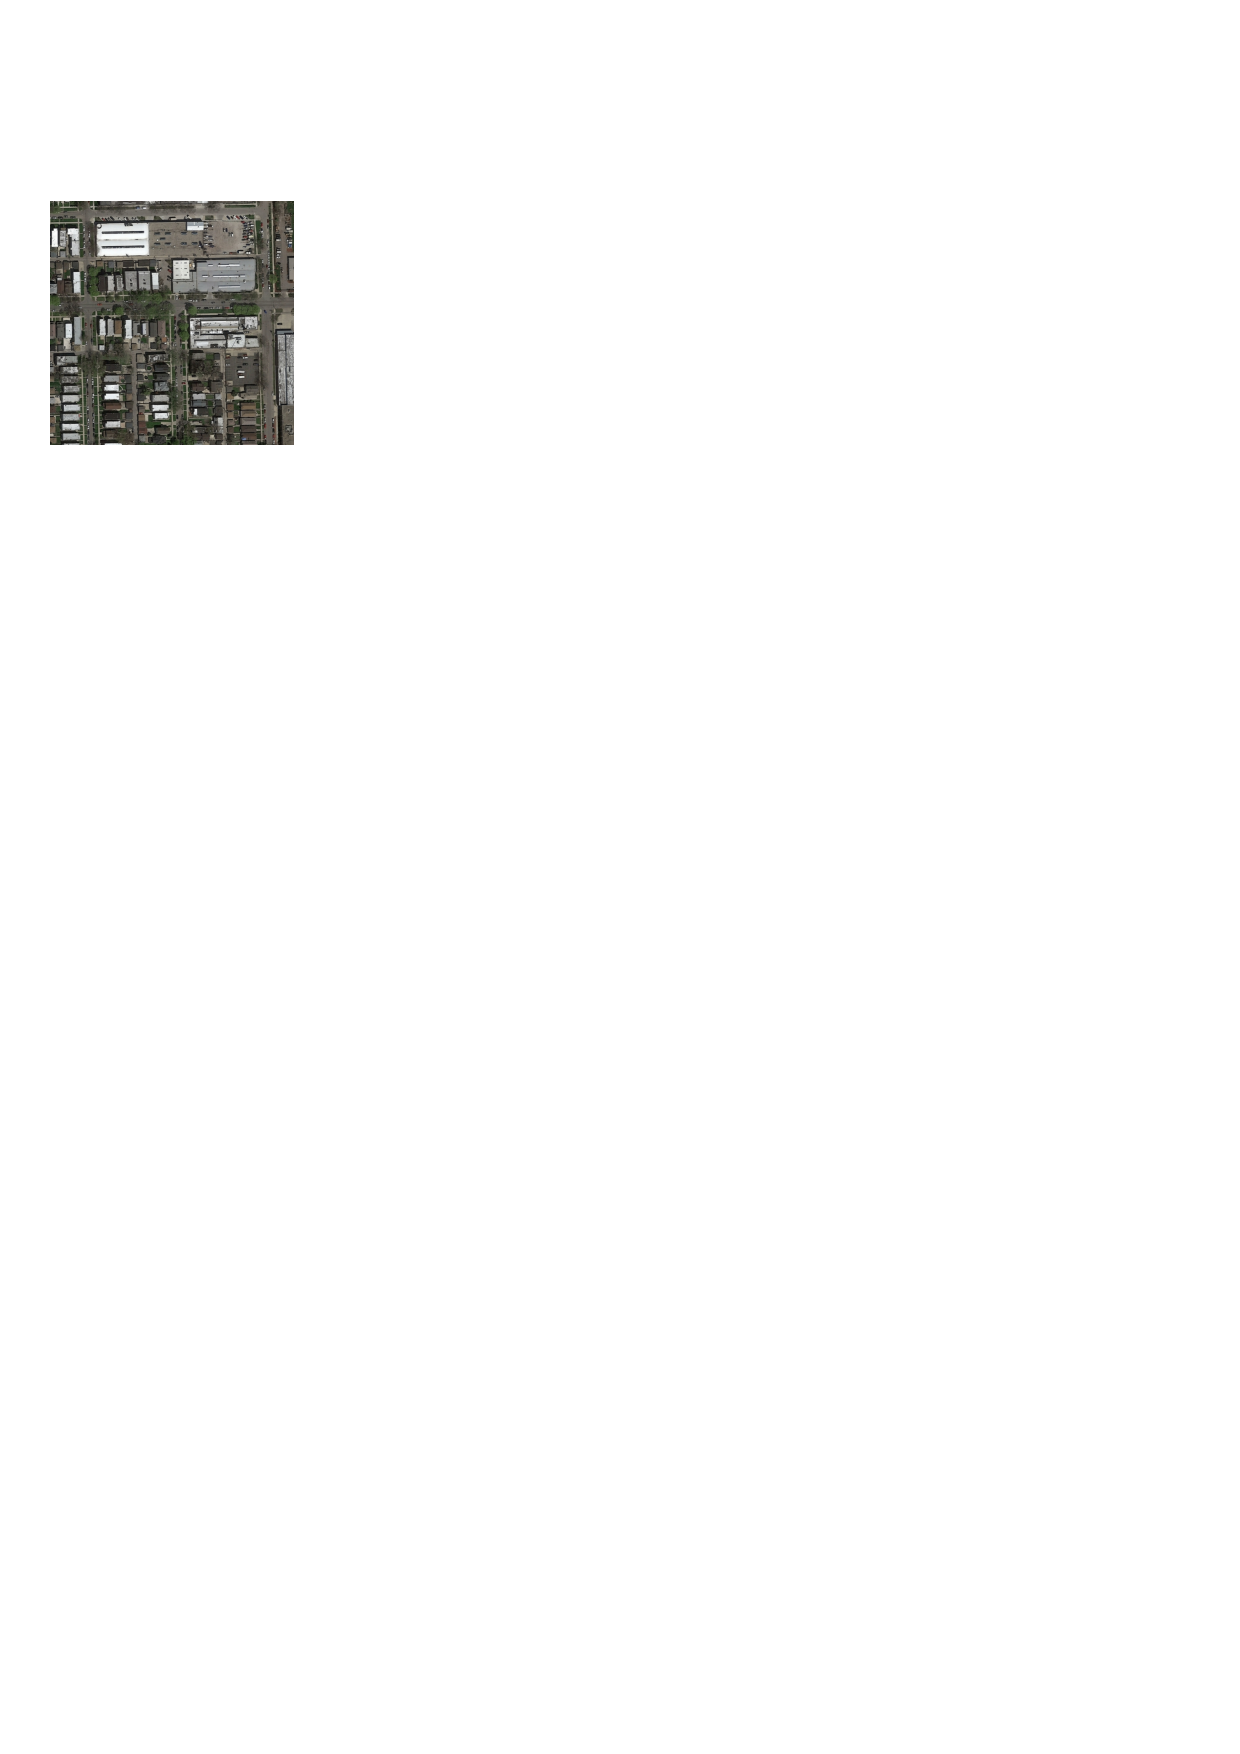
\includegraphics[width=\figfigfigfig\textwidth]{2-00-0.pdf}
	}
	\subbottom[\label{fig:mspascal2}]{
		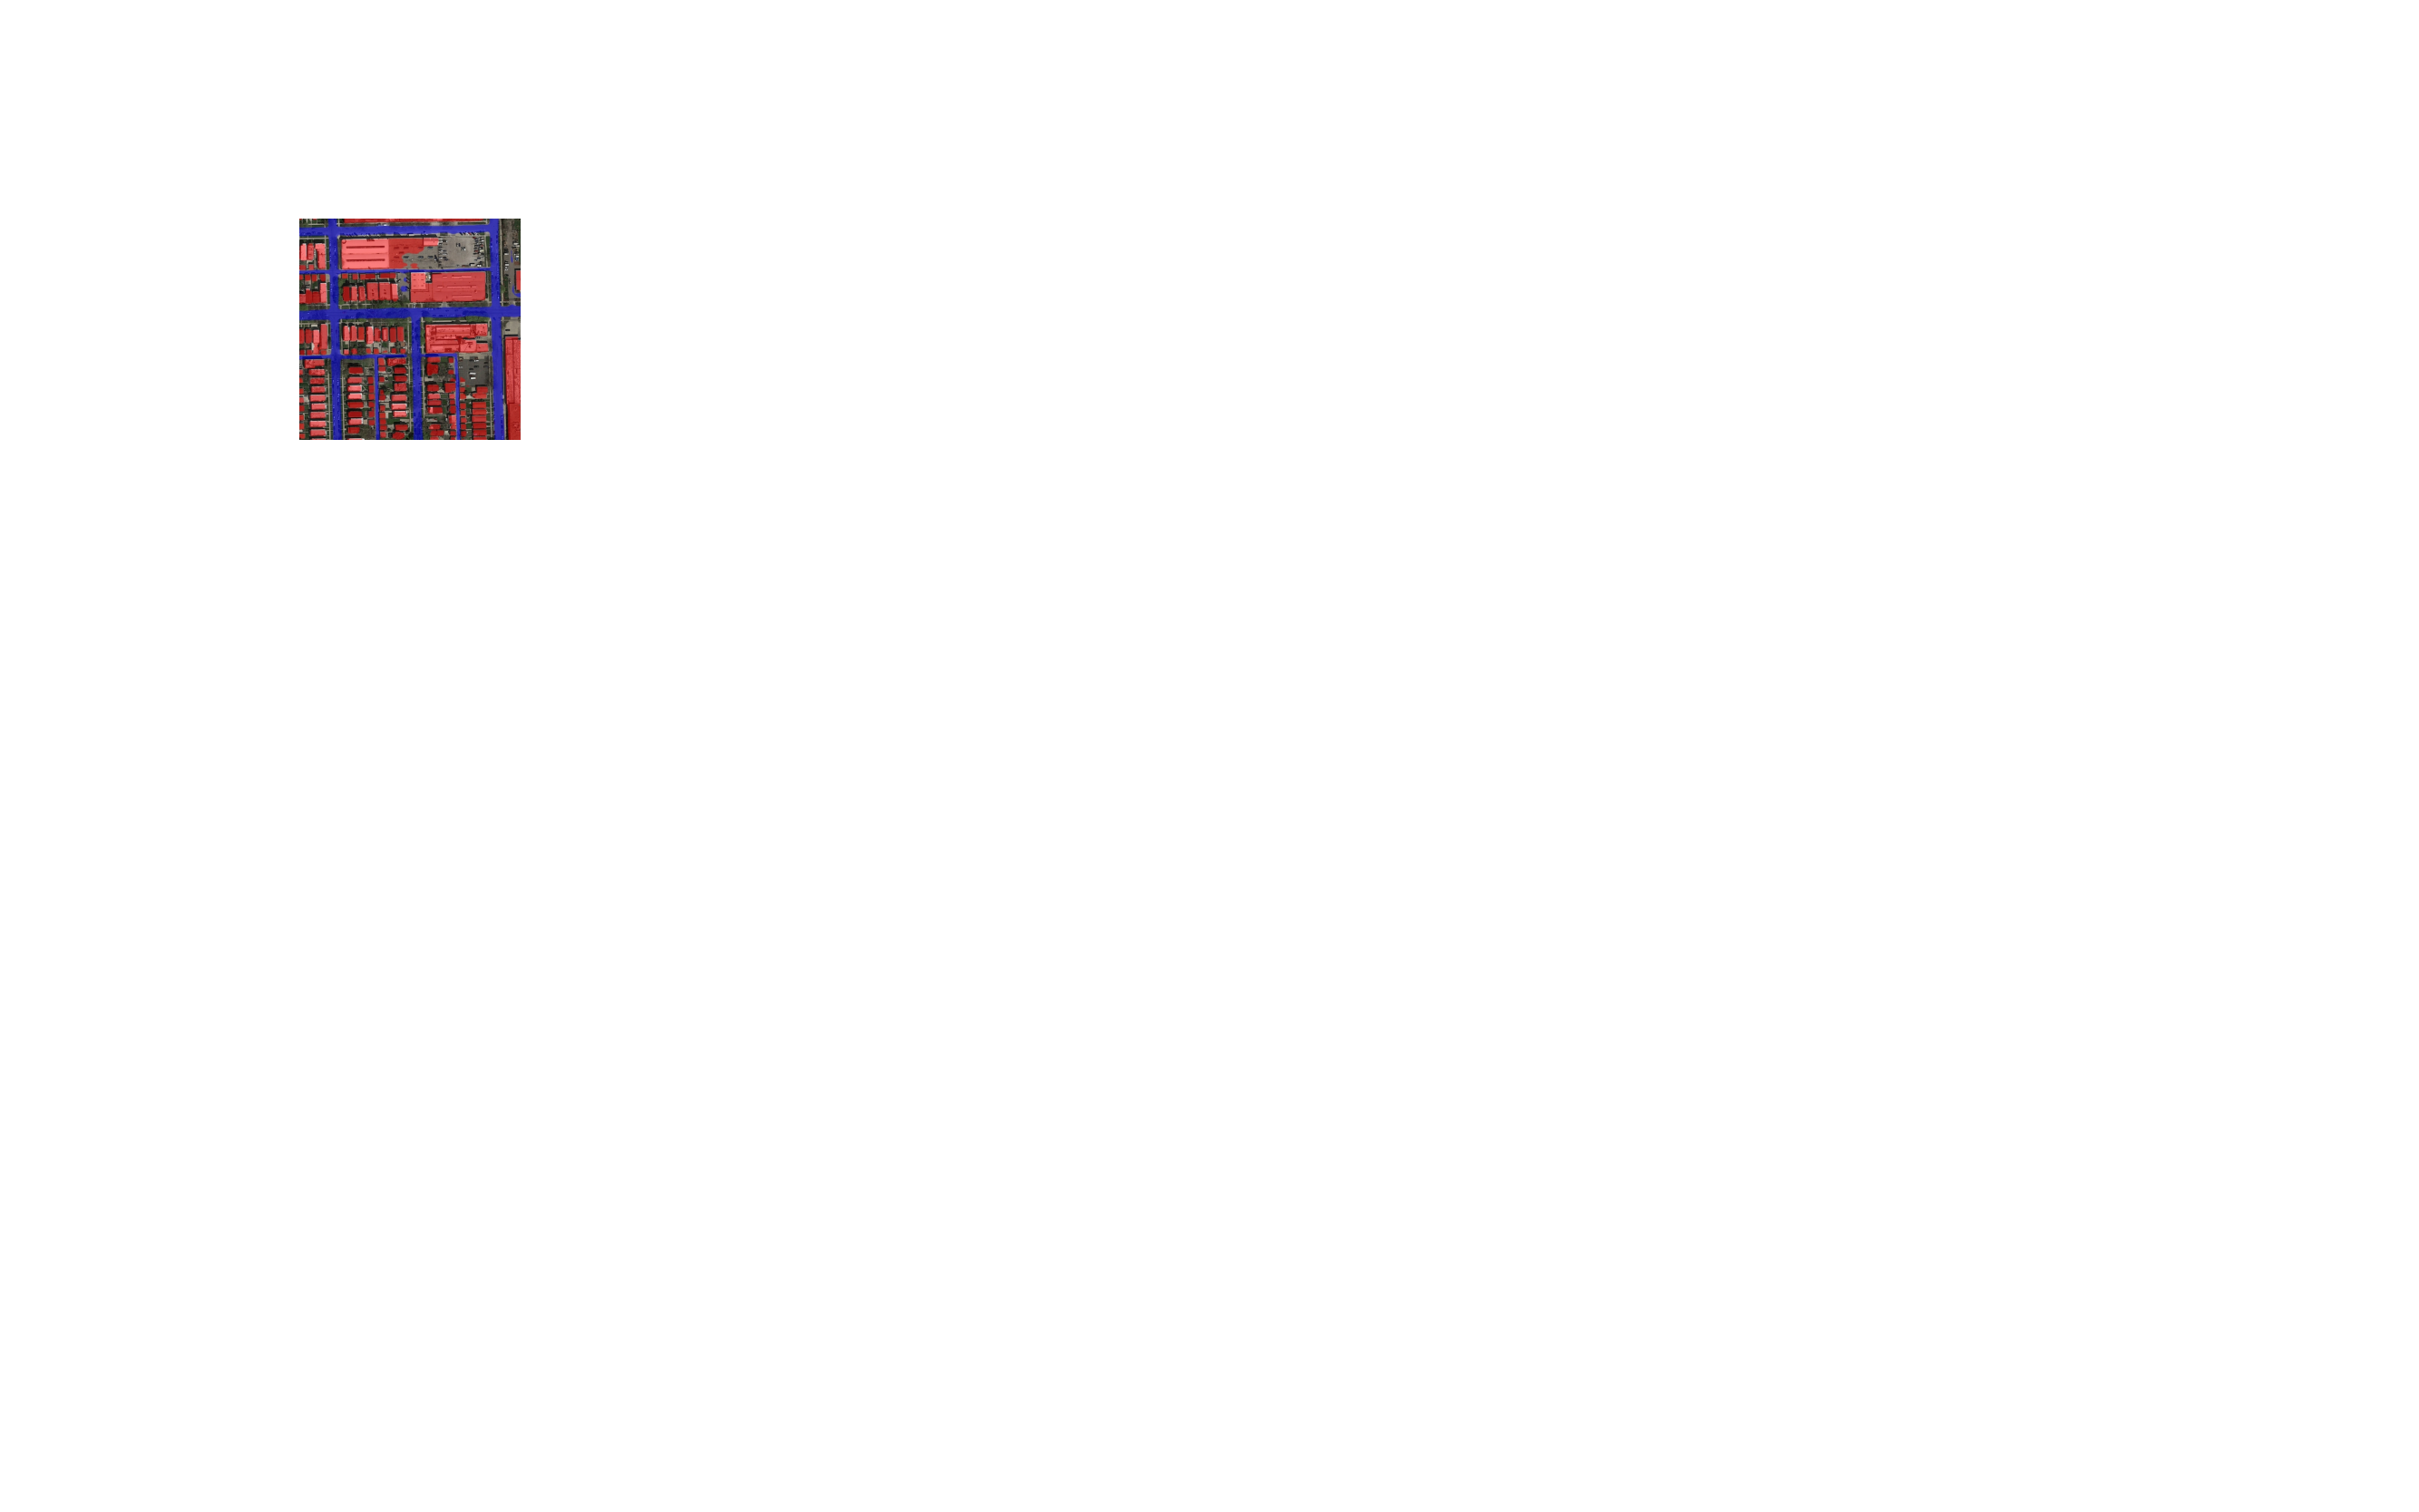
\includegraphics[width=\figfigfigfig\textwidth]{2-00-1.pdf}
	}
	\subbottom[\label{fig:mspascal3}]{
		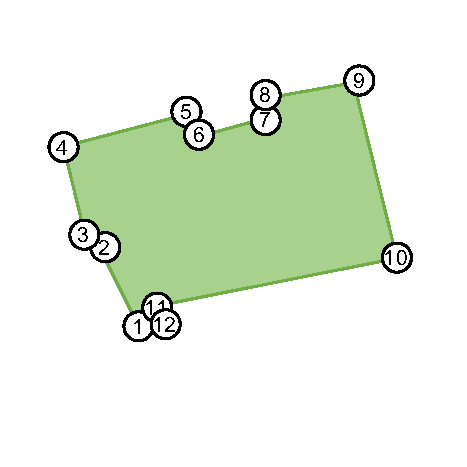
\includegraphics[width=\figfigfigfig\textwidth]{2-00-2.pdf}
	}
	\subbottom[\label{fig:mspascal4}]{
		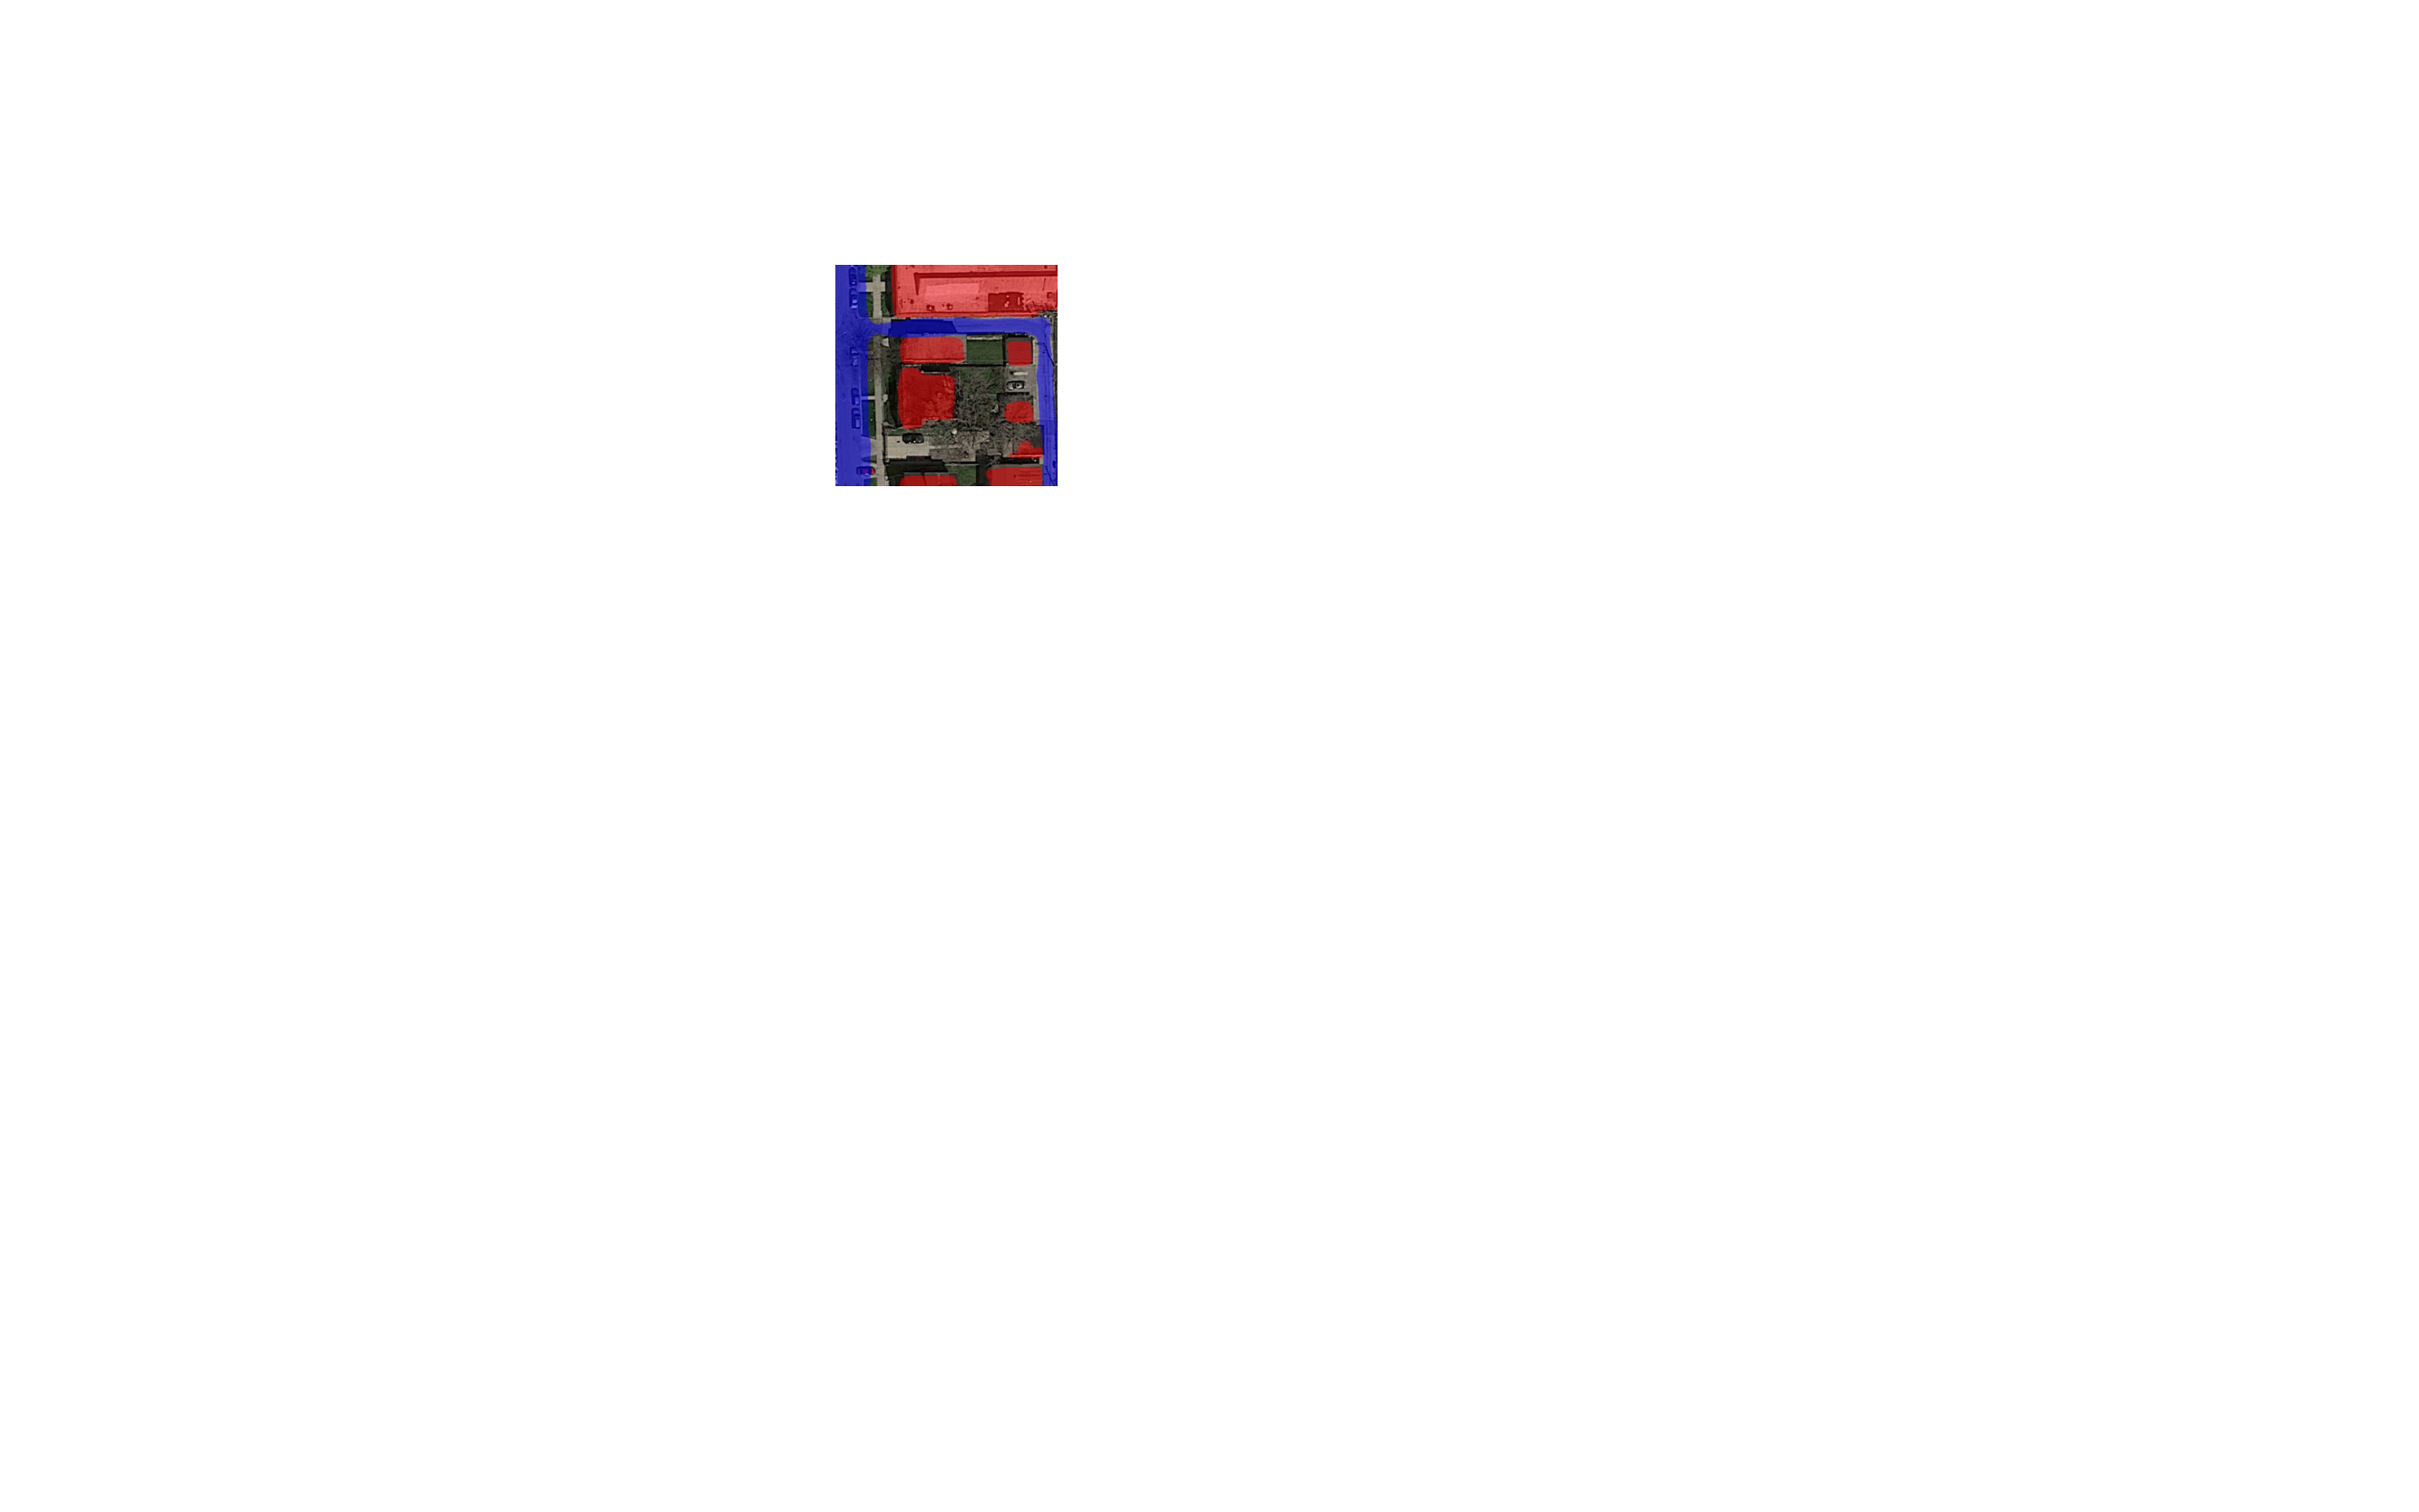
\includegraphics[width=\figfigfigfig\textwidth]{2-00-3.pdf}
	}
    \caption[Semantic segmentation in aerial images]{Semantic segmentation in aerial images. Image copyright owned by \cite{mspascal}. (a) and (c) are two aerial images. In the semantic segmentation result (b) and (d), the pixels covered by red color refer to buildings, while the pixels covered by blue color refer to roads.}
	\label{fig:mspascal}
\end{figure}



We know that predicting a polygon is equivalent to predicting each of its vertices. Thus, the paper regards polygon as a series of vertices, and uses RNN as the model to make coherent prediction. RNN is very powerful when data is related to time series as it can carry complex information about the history. In our case, the prediction of each vertex is dependent on the position of its two previous vertices. The paper also mentioned that another advantage over traditional methods is that RNN can capture the shape of the object even in ambiguous cases like shadows and saturation.

In short, we hope that PolygonRNN can be used to solve our problems, extracting geometric shapes of buildings in aerial images, since the buildings in such images can be also regarded as polygons. For more details of the architecture, please refer to section \ref{modpoly}.

\subsection{Mask R-CNN}\label{relatrcnn}

Dummy text.

\section{Motivation}\label{relatmot}

Dummy text.
